\chapter{Architectuur}\label{ch:Architectuur}
Om bruikbare informatie te kunnen tonen aan de gebruiker moet de informatie dat door de Software Composition Analysis (SCA) Tool wordt geleverd worden bewerkt naar een datamodel waarbij alleen de informatie die relevant is om te tonen wordt opgeslagen. Daarnaast moet het systeem in staat zijn om periodiek een analyse uit te voeren op projecten die bekend zijn binnen de module. In figuur~\ref{fig:SOUP-Components} is te zien hoe onderdelen met elkaar in verbinden staan.
In de secties hieronder wordt ieder onderdeel ver uitgwerkt op een architectonisch niveau.

\begin{figure}[bth]
    \myfloatalign
    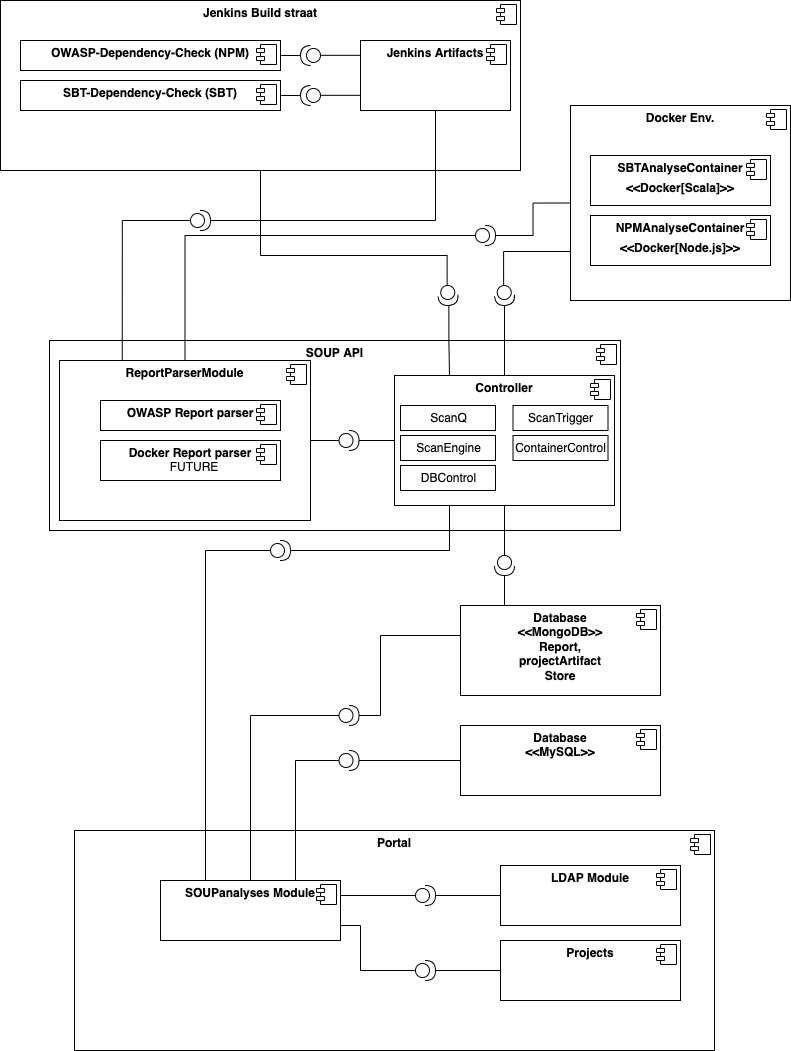
\includegraphics[width=9cm]{gfx/UMLcomponentDiagram}
    \caption{Componenten SOUP Analyse Systeem}
    \label{fig:SOUP-Components}
\end{figure}

\section{SOUPAPI}\label{sec:soupapi}
De SOUP API staat centraal in het nieuwe systeem en is verantwoordelijk voor alle kerntaken die het nieuwe systeem moet uitvoeren. De twee hoofdtaken zijn: "Periodieke scannen van projecten " en "Verwerking van gegevens uit de verkregen resultaten uit de Software Composition Analysis Tool(SCA) en Jenkins, dat gebruikt wordt om een analyse uit te voeren."

\subsection{Verwerking gegevens vanuit de builds}\label{subsec:verwerking-gegevens-vanuit-de-sca}
De belangrijkste taak van de SOUP API is het verwerken van de gegevens die bechikbaar worden gemaakt vanuit een analyse door de SCA Tooling. Deze gegevens komen op twee momenten de applicatie binnen: 1: tijdens het bouwen en deployen van de applicatie. en twee nadat een periodieke scan is geweest

Op het moment dat een project gebuild en/of gedeployed wordt middels de Jenkins Buildstraat moeten nieuwe gegevens over het gebouwde project worden gedeeld met de SOUP API. Deze gegevens bestaan naast meta data over het project, gegevens over de gebruikte dependencies en een rapport dat gegenereerd is door de SCA Tooling.

\begin{figure}[bth]
  \myfloatalign
  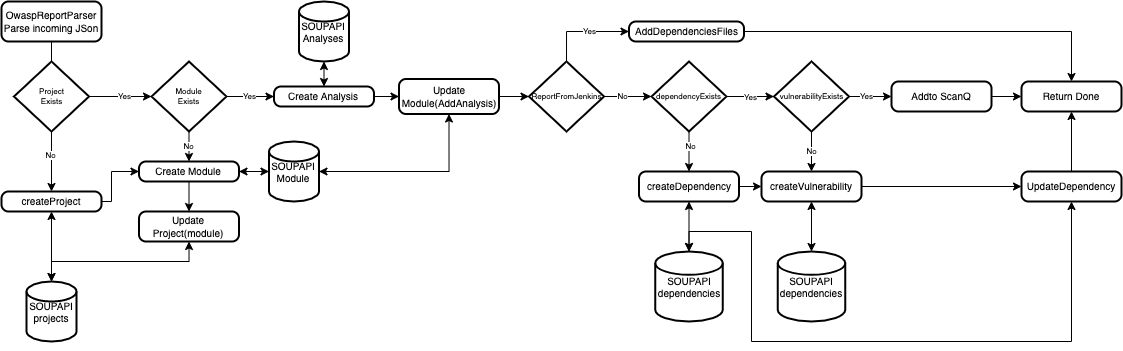
\includegraphics[width=15cm]{gfx/SOUPAPI-ReportParseFlow}
  \caption{Flow van gegevens uit Jenkins naar de SOUP API}
  \label{fig:SOUP-ReportPArseFlow}
\end{figure}

In figuur~\ref{fig:SOUP-ReportPArseFlow} is een globale beschrijving van een flow te zien hoe de data die uit de jenkins buildstraat komt wordt verwerkt. De data komt binnen middels een CURL command dat afgevuurdt wordt in de pipeline van Jenkins( wordt beschreven in de sectie over Jenkins).
De Dependency service is verantwoordelijk voor het borgen van de dependency informatie. Hier wordt iedere keer als er een build/deploy is geweest de dependency informatie toegevoegd aan de betreffende module. Op deze manier kan de periodieke scanner deze informatie gebruiken om op een later moment herhaaldelijk de project dependencies te scannan op kwetsbaarheden.




Voor de verwerking van informatie is de ReportParser verantwoordelijk  Het wordt in gezet voor het vertalen en omzetten van de data uit rapporten die door de SCA Tooling worden gegenereerd naar data die gebruikt worden binnen de SOUP-module van de portal. In dit ontwerp is er een parser aanwezig voor het vertalen van de OWASP-engine rapporten\footnote{De SCA tooling in het vorige hoofdstuk genereren beide rapporten in het zelfde JSON schema}. In de toekomst zullen er meerdere parsers moeten worden toegevoegd op het moment dat er een andere runtime wordt meegenomen welke niet door de OWASP engine kunnen worden gescanned.

De Controller is verantwoordelijk voor de taken die te maken hebben met het periodiek scannen van projecten Het heeft faciliteiten zoals een scanQ waarin de projecten staan die gescanned moeten worden. Een analyser die op het moment dat een project aan de beurt is om geanalyseerd te worden een aantal subtaken sequentieel uitvert per module binnen een project.
In grote lijnen wordt er een dockercontainer opgezet per module waarin alle benodigde bestanden (dependency declaraties en dergelijke) worden geplaats. Vervolgens een analyse wordt uitgevoerf waaruit de resultaten naar de ReportParser kan worden gestuurt voor analyse. De exacte werking wpordt verderop in het document technisch uitgewerkt.

\section{Jenkins buildtstraat}\label{sec:jenkins-buildtstraat}
Op het moment dat er een project wordt gebouwd middels de Jenkins buildstraat kan er vanuit worden gegaan dat er wijzigingen zijn in de sourcecode. Mogelijk zijn er dan ook wijzigingen in de declaraties in bijvoorbeeld versies en of nieuwe of andere dependencies de gebruikt worden. In het nieuwe systeem wordt Jenkins gebruikt om deze informatie in het systeem te verkrijgen. Om deze informatie in de SOUP API te krijgen moeten er een aantal aanpassingen gedaan worden die ervoor zorgen dat informatie omtrend kwetsbaarhden in een uniforme manier worden gewonnen en verstuurd naar de SOUP API.

\subsection{Data}\label{subsec:jenkins_Datamodel}
De informatie die uit Jenkins wordt verkregen is informatie waarop op een later moment de periodieke analyses worden gebaseerd. De data die verstuurt wordt moet dan ook het volgende bevatten: Data over de identiteit van het project en welke modulen er aanwezig zijn. De rapporten die gegenereerd zijn door de in de pipeline aanwezige analyse tools. En de dependencies die gebruikt worden. Om de data in een zo universeel mogelijke manier te versturen wordt het data transfer model genbruitk die in listing \ref{lst:DTMJenkins} te zien is. Het model bestaat uit drie hoofddelen waarin de gegevens over de analyse en het project zijn opgeslagen, De Rapporten die gegenereerd worden door de SCA tooling ingebouwd in de pipeline waarbij ook de tool is meegegeven. En van iedere module een lijst met dependencies.
\begin{lstlisting}[caption={Data transfer model vanuit Jenkins},label=lst:DTMJenkins]
{
  "projectnaam": "GroeiGids",
  "BuildHash": "fb5f5cb47bbd0cbf2f4771c55242fedbf41c5efc",
  "buildDate": "22-01-2022",
  "buildModules": [
    "App",
    "portal",
    "backend"
  ],
  "reports": [
    {
      "NPM-portal-report": {
        "tool": "OWASP-NPM",
        "report": {}
      }
    },
    {
      "NPM-app-Report": {
        "tool": "OWASP-NPM",
        "report": {}
      }
    },
    {
      "sbt-backend-report": {
        "tool": "OWASP-SBT",
        "report": {}
      }
    }
  ],
  "dependencies": [
    {
      "npm-portal-deps": {
        "dependencies": [
          {
            "naam": "<<NAAM>>",
            "versie": "<<Versie>>"
          }
        ],
        "devDependencies": [
          {
            "naam": "<<NAAM>>",
            "versie": "<<Versie>>"
          }
        ]
      }
    },
    {
      "npm-app-deps": {
        "dependencies": [
          {
            "naam": "<<NAAM>>",
            "versie": "<<Versie>>"
          }
        ],
        "devDependencies": [
          {
            "naam": "<<NAAM>>",
            "versie": "<<Versie>>"
          }
        ]
      }
    },
    {
      "sbt-backend-deps": {
        "dependencies": [
          {
            "naam": "<<NAAM>>",
            "versie": "<<Versie>>"
          }
        ]
      }
    }
  ]
}
\end{lstlisting}

\subsection{informatie extractie methoden en verzending van de informatie}

Voor iedere module in een project moet de betreffende SCA tool worden aangeroepen waatbij het Rapport wordt toegevoegd aan de Jenkins Artifacts.
Op het moment dat de deploy gedaan is moeten deze rapporten samen worden gevoegd met de metadata tot een JSON bestand welke vervolgens middels een POST methode kan worden vertuurt naar de SOUP API welke het vervolgen middels de Parser toevoegd aan de database en scheduler als zijn een bestaand project die periodiek moet worden geanalyseerd.

\section{Portal}\label{sec:portal}
In de portal wordt er een module toegevoegd die als interface dient voor het SOUP-analyse systeem. Informatie over kwetsbaarheden in geanalyseerde projecten worden hier weergegeven. Ook is het hier mogelijk om per project in te kunnen zien welke instellingen er gelden voor analyses en waar zo nodig kunnen deze hier worden aangepast.
In de module moet er dus een plek komen waar informatie betreft kwetsbaarheden kan worden geraadpleegd. Daarnaast moet en er een plek komen waarbij instellingen kunnen worden aangepast zodat de analyses worden uitgevoerd op de ingesteld periode. En of aan en uit gezet kan worden.

In de komende hoofdstukken zullen de dir ehoofd modulen verder worden uitgwerkt in een functioneel ontwerp
